Para entender la señal del proceso \MSSM\textbf{D} (estos procesos corresponden con la descomposición según lo muestra el diagrama de la Fig. \ref{fig:sketch_darksector}), siendo el objetivo de estudio en esta investigación, se hace necesario su caracterización antes y después de simular su paso por las diferentes configuraciones del detector. Conocer la morfología de la señal real y la reconstruida por el detector nos permitirá comprender la teoría y como está es visualizada por el experimento \CMS.

\subsection{Variación del contenido muónico}

Se hace hace necesario investigar el contenido muónico de la señal \MSSM\textbf{D}~ bajo las diferentes condiciones de generación, para hacer referencia a estas condiciones iniciales con las que se generó la señal, se hará uso del vector:
\begin{equation}
\vec{\alpha} = (m_{n_1}, m_{n_D}, m_{\gamma_D}, c\tau_{\gamma_D})
\end{equation}
además el número de partículas $p$ en el i-ésimo evento generado está definido por:
\begin{equation}\label{numero_particulas}
n_i^{(p,k)} \equiv n_i^{(p,k)} (\vec{\alpha})
\end{equation}
donde 
$k =$ \begin{small}$\textsf{R2},~\textsf{HL}, ~\textsf{True}$\end{small}  declara la presencia del detector y su configuración, 
$i = 1, \ldots, N_{e}$ hace referencia al evento y 
$p = \mu^\pm, ~ \gamma_D, ~n_D, ~n_1$ partícula caracterizada.
%\begin{tabular}{lll}
%$k$ & $= \textsf{R2},~\textsf{HL}, ~\textsf{True}$ & declara la presencia del detector y su configuración.\\
%$i$ & $ = 1, \ldots, N_{e}$ & hace referencia al evento.\\
%$p$ & $ = \mu^\pm, ~ \gamma_D, ~n_D, ~n_1$ & partícula caracterizada.
%\end{tabular}
Definiendo a $f^{(p, k)}_\textsf{e} (x)\equiv f^{(p, k)}_\textsf{e} (x; \vec{\alpha})$ como la fracción del total de eventos poseedores de un número $x$ de partículas tipo $p$ de la señal generada bajo las condiciones iniciales $\vec{\alpha}$ y con la configuración del detector $k$ se tiene entonces:
%\mathbb{M} 
\begin{equation}\label{fe}
f^{(p, k)}_\textsf{e} (x)  = \dfrac{\sum\limits_{i=1}^{N_e} \delta_{x,n_i^{(p,k)}}}{\sum\limits_{i=1}^{N_e} \sum\limits_{x=0}^\infty \delta_{x,n_i^{(p,k)}}} = \dfrac{1}{N_e} \sum_{i=1}^{N_e} \delta_{x,n_i^{(p,k)}}
\end{equation}
donde $x\in\mathbb{N}$ pertenece al grupo de lo números naturales, $\delta_{x,n_i^{(p,k)}}$ es la función delta de Kronecker. Por otro lado $\mathbb{F}^{(p, k)}_\textsf{e} (x)\equiv \mathbb{F}^{(p, k)}_\textsf{e} (x; \vec{\alpha})$ es la fracción del total de eventos que contienen muones de ruido no procedentes del decaimiento de la señal \MSSM\textbf{D}, dada por:
\begin{equation}\label{fnInverso}
\mathbb{F}^{(p, k)}_\textsf{e} (x)= 1 - f^{(p, k)}_\textsf{e}  (x; \vec{\alpha})
\end{equation}
% ~~~ y ~~~ ff^{(p, k)}_\textsf{e} (\vec{\alpha}; x) = 1- f^{(p, k)}_\textsf{e} (\vec{\alpha}; x)
Finalmente, $f^{(p, k)}_\textsf{n} (\vec{\alpha}; x)$ es la fracción de partículas tipo $p$ que se encuentran en eventos con $x$ de estás partículas:
\begin{eqnarray}\label{fn}
f^{(p, k)}_\textsf{n} (x; \vec{\alpha}) & = \dfrac{\sum\limits_{i=1}^{N_e} n_i^{(p,k)} \delta_{x,n_i^{(p,k)}}}{\sum\limits_{i=1}^{N_e} \sum\limits_{n=0}^\infty n_i^{(p,k)} \delta_{n, n_i^{(p,k)}}}  = \dfrac{\sum\limits_{i=1}^{N_e} n_i^{(p,k)} \delta_{x, n_i^{(p,k)}}}{\sum\limits_{i=1}^{N_e} n_i^{(p,k)}}
\end{eqnarray}

%\begin{equation}
%\Delta f^{(\geqslant 4\mu, \backsim)}_\textsf{rel} = \left[ \sum_{i,n} \mathbb{E}_i^{(n\mu, \backsim)} - \sum_i \mathbb{E}_i^{(4\mu, \backsim)} \right]/\sum_{i,n} \mathbb{E}_i^{(n\mu, \backsim)}
%\end{equation}
%\begin{equation}
%\Delta f^{(\geqslant 4\mu, \backsim)}_\textsf{n} = \left[ \sum_{i,n} n \cdot \mathbb{E}_i^{(n\mu, \backsim)}- \sum_i 4 \cdot \mathbb{E}_i^{(4\mu, \backsim)}\right]/\sum_{i,n} n \cdot \mathbb{E}_i^{(4\mu, \backsim)}
%\end{equation}
%\begin{equation}
%\Delta f^{(\geqslant 4\mu, \textsf{True})}_\textsf{n} = \left[ \sum_{i} n^{(\mu,\textsf{True})}_i \cdot \mathbb{E}_i^{(\textsf{True})} \cdot (1- \textsf{IO}(n^{(\mu,\textsf{True})}_i,~ 4) \right]/\sum_{i} n^{(\mu,\textsf{True})}_i \cdot \mathbb{E}_i^{(\textsf{True})} 
%\end{equation}

Algunos ejemplos del contenido muónico de los eventos se pueden mostrar en la Fig. \ref{contenido_muonico}, donde se puede visualizar los cambios dependientes del parámetro de generación masa del fotón oscuro $m_{\gamma_D}$. Se constató en la investigación de la señal, la invarianza de la distribución del contenido muónico por evento ante los cambios de la masa del neutralino oscuro $m_{n_D}$ y del tiempo de vida del fotón oscuro $c \tau_{\gamma_D}$, cuestión esperada por la teoría, ya que son elementos que no se esperan estar relacionados con los procesos de ruido que generen muones.

\begin{figure}[!ht]
\centering
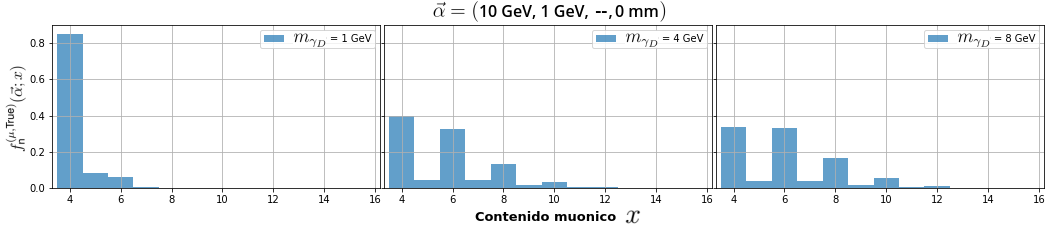
\includegraphics[width=1\textwidth]{Simulacion/imagenes/True_Entries.png}
\caption{Variación del contenido muónico de los eventos antes de pasar por el detector.}
\label{contenido_muonico}
\end{figure}

De la Fig. \ref{contenido_muonico} se conoce que el contenido mínimo de muones por evento para $k=\textsf{True}$ es de 4 muones, estos son el resultado de la recreación de la señal \MC ~ proveniente de \MSSM\textbf{D} relacionada con el decaimiento de la Fig. \ref{fig:sketch_darksector}b. Algunos ejemplos de variación de la fracción de eventos con muones provenientes de señales de ruido $\mathbb{F}^{(\mu, \textsf{True})}_\textsf{e}(4)$ y de la fracción  de muones provenientes de señales de ruido $1- \frac{4 N_e}{\sum n_i^{(p,k)}}$ (todos los eventos generados por \MC ~ en Madgraph contienen el decaimiento de la Fig. \ref{fig:sketch_darksector}b) se muestran en la Tabla \ref{generacion0}.


% \multicolumn{4}{cccccc}{Parámetros de generación ($\vec{\alpha}$)}
\begin{table}[!h]
\centering
\begin{tabular}{|cccc|c|c|}
\toprule
\multicolumn{4}{|c|}{Parámetros de generación ($\vec{\alpha}$)} & \multicolumn{2}{|c|}{Variables} \\
\midrule
$m_{n_1}$  & 
$m_{n_D}$ & 
$m_{\gamma_D}$ & %$\textsf{(GeV)}$ 
$c\tau_{\gamma_D}$  & %$\textsf{(mm)}$
$\mathbb{F}^{(\mu, \textsf{True})}_\textsf{e}(4)$ ($\textsf{\%}$)&
$1- \dfrac{4 N_e}{\sum\limits_{i=1}^{N_e} n_i^{(p,k)}}$ ($\textsf{\%}$)\\
\midrule
10 & 1 & 1 & 0 & 15.32 & 5.50 \\
10 & 1 & 4 & 0 & 60.43 & 30.16\\
10 & 1 & 8 & 0 & 66.16 & 34.08\\
\bottomrule 
\end{tabular}%}
\caption{Cambio del contenido muónico de procesos con variación de la masa de fotón oscuro $m_{\gamma_D}$.}
\label{generacion0}
\end{table}
Al analizar los resultados obtenidos, se pudo concluir que hay un aumento del ruido muónico en la reconstrucción de la señal \MSSM\textbf{D} con el aumento teórico del parámetro de generación correspondiente a la masa del fotón $m_{\gamma_D}$ (ver Tabla \ref{generacion0}), sin embargo no se observan cambios con el cambio de los parámetros $m_{n_D}$ y $c\tau_{\gamma_D}$. Los datos que se poseen no son adecuados para estudiar la correspondencia con la masa del neutralino ligero $m_{n_1}$.

\subsection{Variación de las propiedades de los muones con el parámetro $\vec{\alpha}$}

Analizar la señal \textbf{Dark}-\SUSY ~o \MSSM\textbf{D}~ mediante las propiedades de los muones sin la reconstrucción del detector dará una base de comparación y un mayor entendimiento de la teoría. Además, separar la información según los muones que provienen del decaimiento $h \rightarrow 2n_1 \rightarrow 2n_D + 2\gamma_D \rightarrow 2n_D + 4\mu$ del resto de los procesos se hace necesario para una mejor interpretación de la reconstrucción conjunta de las señales. Se introduce la notación de las propiedades de una partícula $p= n_1, ~n_D, ~\gamma_D, ~\mu$, siendo la distribución de frecuencia dada por:
\begin{equation}\label{Wpk}
\textsf{W}^{(p,k)} (\chi) \equiv \textsf{W}^{(p,k)} (\chi; \vec{\alpha}) ~~~~~~ \longrightarrow ~~~~~~ \textsf{W}^{(p,k)}_N (\chi) = \dfrac{\textsf{W}^{(p,k)} (\chi)}{ \sum\limits_\chi \textsf{W}^{(p,k)} (\chi)}
\end{equation}
donde $\chi$ hace referencia a la propiedad de interés, estás se pueden ver en la Tabla \ref{propiedades}.

\begin{table}[!h]
\centering
\begin{tabular}{|p{1.2cm}|p{13cm}|}
\toprule
$\chi$ & Definición\\
\midrule
$m$ & Masa invariante\\
$PT$ & Momento de la partícula%, normalmente referenciada por su proyección en dirección transversal \texttt{\textbf{PZ}} $=$ \texttt{\textbf{P}} $\sin \theta$, donde $\theta$ es el ángulo polar, definido como aquel entre el vector momento y la dirección positiva del as, normalmente utilizado ya que no es invariante frente a transformaciones de Lorentz
.\\
$\eta$ & Pseudoapidez, esta representa la coordenada espacial que describe el ángulo de una partícula en relación con el eje del haz. Su ecuación tiene la forma:
\begin{equation}
\eta = -\ln \left[ \tan \left( \dfrac{\theta}{2} \right)\right]
\end{equation}\\[-1cm]
$\phi$ & Ángulo azimutal.\\
$c\tau$ & Tiempo de vida media, esta describe la descomposición de las partículas, se expresa comúnmente en términos de vida media, constante de descomposición o vida media. \\

$D_0$ & Parámetro de impacto transversal, se define como la distancia transversal al eje del haz en el punto de máxima aproximación, donde su signo esta dado de acuerdo al momento angular de la traza alrededor de eje.\\

$D_Z$ & Parámetro de impacto longitudinal, definido como la posición de la coordenada $z$ de la traza en el punto de maximo acercamiento.\\
\begin{small}$\textsf{Sum}Pt$\end{small} & Variable de aislamiento basada en el rastreador de partículas, se define como la suma escalar del $PT$ de las partículas en el plano $\eta \times \phi$ dentro de un cono $\Omega$\\
$Iso$ & Combinación del aislamiento de \textbf{ECAL}, \textbf{HCAL} (ver sección \ref{Experimento_CMS}) y \begin{small}$\textsf{Sum}Pt$\end{small}.\\

%\item[-] \texttt{SumPtNeutral}: xxx\\
%\item[-] \texttt{SumPtCharged}: xxx\\
\bottomrule
\end{tabular}
\caption{Propiedades y definiciones de las partículas.}
\label{propiedades}
\end{table}

\begin{figure}[!ht]
\centering
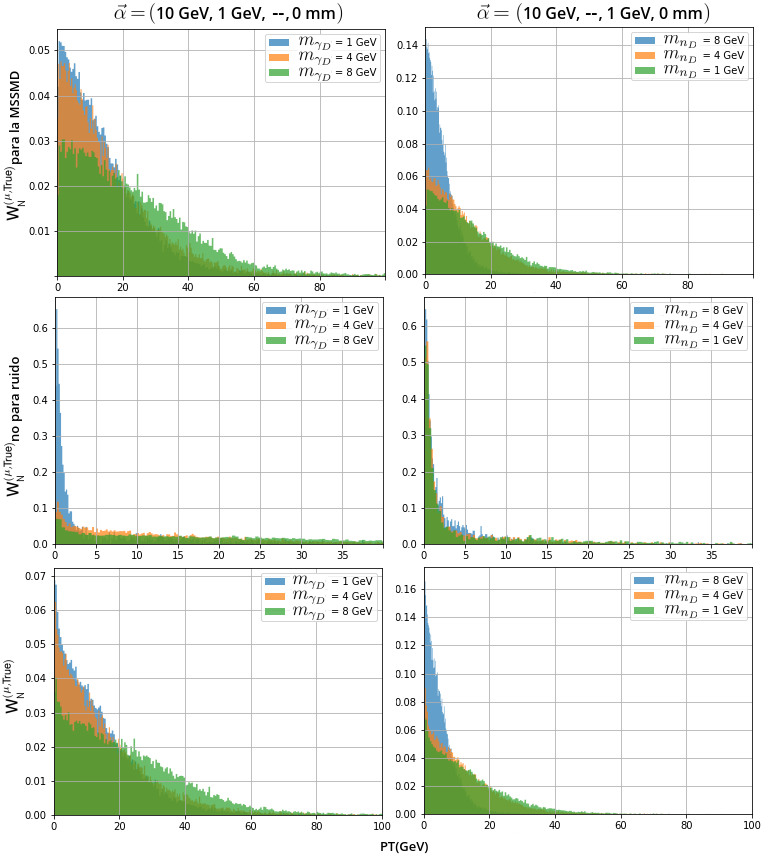
\includegraphics[width=.9\textwidth]{Simulacion/imagenes/True_PT4.png}
\caption{Variación de las distribuciones de los momentos transversales de los muones .}
\label{PT_mu_True}
\end{figure}

La distribución correspondiente al momento transversal de los muones $\textsf{W}^{(\mu,\textsf{True})}_N (PT)$ proveniente del decaimiento  \textbf{Dark-}\SUSY ~ (\MSSM\textbf{D}),
de otros procesos secundarios o ruido y la unificación de todas se pueden visualizar en la Fig. \ref{PT_mu_True}. Con la comparación de las distribuciones se pudo evidenciar la variación de su morfología con el cambio del parámetro de generación masa del fotón oscuro $m_{\gamma_D}$ y del neutralino oscuro $m_{n_D}$. 


Las distribuciones muestran que el $\sim 95$\% de los muones correspondientes al decaimiento \MSSM\textbf{D} ~ muestran su dominio para valores $PT < 80 \textsf{ GeV}$, para los muones resultantes de procesos de ruido tenemos $PT < 10 \textsf{ GeV}$. Además, se confirma una relación directa entre los estadísticos medios del momento transversal de los muones con el parámetro de generación masa del fotón oscuro $m_{\gamma_D}$, de forma inversa con el parámetro de masa del neutralino oscuro $m_{n_D}$.


\subsection{Características del fotón oscuro $\gamma_D$}
La reconstrucción del fotón oscuro $\gamma_D$ predicho por el decaimiento \MSSM\textbf{D} es el motivo principal de estudio de esta investigación. La caracterización de sus propiedades y el cambio de la morfología de los gráficos de frecuencias $\textsf{W}^{(\gamma , \textsf{True})}_N (\chi)$ con el cambio de los parámetros de generación $\vec{\alpha}$, permitirá una comprensión mas completa de los resultados obtenidos con la reconstrucción realizada por los detectores en la configuración Run-2 ($\textsf{R2}$) y Alta Luminosidad ($\textsf{HL}$).


\begin{figure}[!h]
\centering
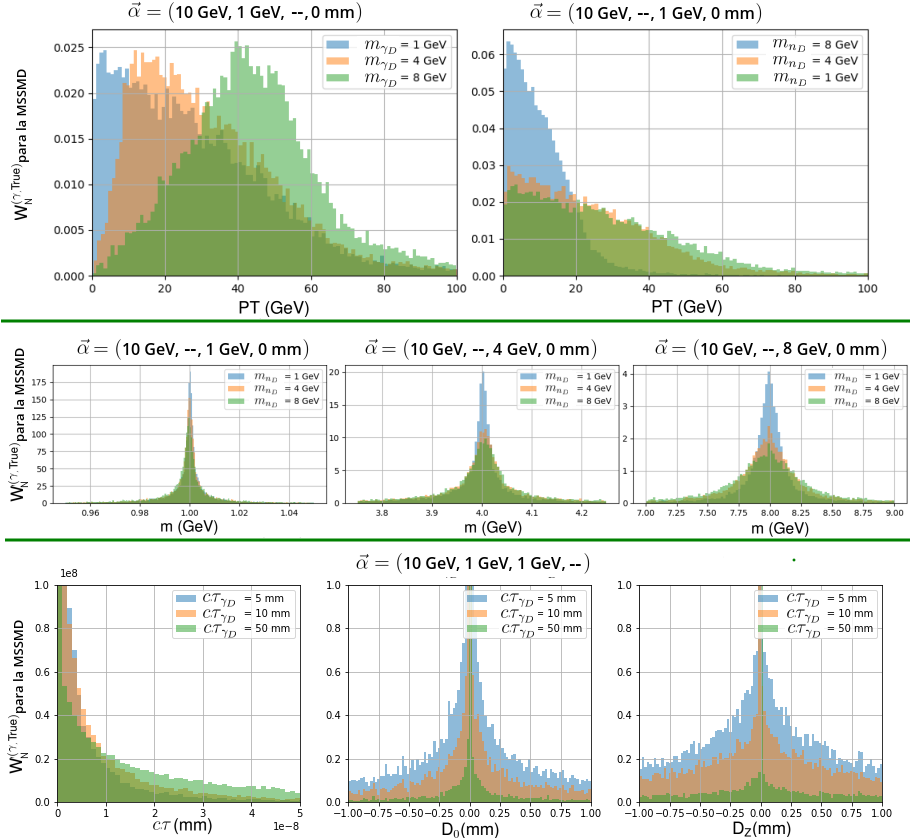
\includegraphics[width=.9\textwidth]{Simulacion/imagenes/True_PT5.png}
\caption{Variación de las propiedades del fotón oscuro $\gamma_D$ con los parámetros de generación $m_{\gamma_D}$, $m_{n_D}$ y $\tau c_{\gamma_D}$.}
\label{PT_mu_True2}
\end{figure}

Los gráficos de la Fig. \ref{PT_mu_True2} muestra la clara dependencia del momento angular $PT$ y con los parámetros de masa de $\vec{\alpha}$, ya que son la masa del fotón $m_{\gamma_D}$ y su tiempo de vida $c\tau_{\gamma_D}$ son tratados por la teoría como parámetros libres, no hay dependencia directa entre ellas. Hay una correspondencia clara entre los parámetros de impacto $D_\textsf{0}$ y $D_\textsf{Z}$ como se esperaría con el parámetro de generación $c\tau_{\gamma_D}$.


\subsection{Identificando y reconstruyendo el fotón oscuro $\gamma_D$}

Es de gran interés en esta investigación la creación de una metodología de identificación de di-muones, que pueda discernir entre los muones provenientes de la señal \MSSM\textbf{D}, emparejarlos y reconstruir correctamente el fotón oscuro del cual teóricamente se espera que hayan decaído según el diagrama de la Fig. \ref{fig:sketch_darksector}b. Esta herramienta de identificación, puede crearse, haciendo uso de las redes artificiales neuronales, ya que la misma posee altas capacidades de aprendizaje, generalización, adaptación y tolerancia a fallos, haciéndola una herramienta robusta en el reconocimiento de patrones y objetos.     .

\begin{figure}[!h]
\centering
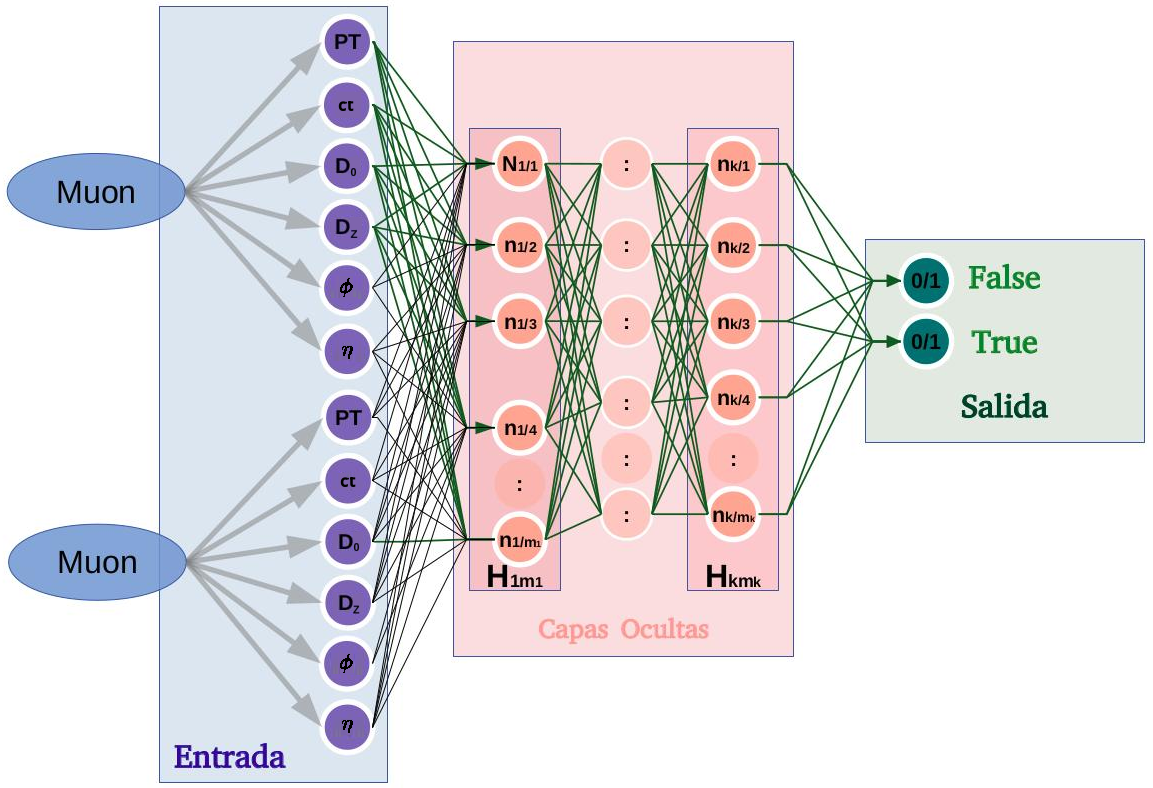
\includegraphics[width=.9\textwidth]{Simulacion/imagenes/IDENTIFICADOR.png}
\caption{Diagrama de la estructura de la red neuronal dedicada a la identificación de di-muones provenientes del fotón oscuro $\gamma_D$.}
\label{identificador}
\end{figure}

Se crea una red artificial que dadas las propiedades de los di-muones, pueda informar si esta selección proviene o no de un fotón oscuro de \MSSM\textbf{D} (ver Fig. \ref{identificador}). Este problema, es equivalente al perceptrón simple, siendo una de las caracterizaciones más básicas en el área de redes neuronales artificiales.
Para implementar este identificador se hace uso de las paqueterías o herramientas de $\textsf{keras}$ programando en el entorno de \textbf{Python}.

El modelo genérico de neurona artificial se puede ver en la Fig. \ref{generico}, en este se puede visualizar el funcionamiento simple de una neurona en forma de un procesador elemental, que a partir de un vector de entrada procedente del exterior o de otras neuronas, proporcionando una única respuesta o salida.

\begin{figure}[!h]
\centering
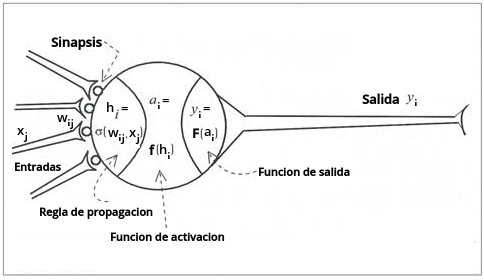
\includegraphics[width=.7\textwidth]{Simulacion/imagenes/generico.png}
\caption[Modelo genérico de una neurona artificial.]{Modelo genérico de una neurona artificial.\footnote{Página de origen: \href{https://grupo.us.es/gtocoma/pid/pid10/RedesNeuronales.htm}{https://\-gru\-po.\-us.\-es/\-gto\-coma/\-pid/\-pid10/\-Re\-des\-Neu\-ro\-na\-les.\-htm}}}
\label{generico}
\end{figure}

Los elementos que constituyen neurona genérica se pueden observar en la Fig. \ref{generico}, siendo $x_i(t)$ las variables de entrada y salida, los pesos sinápticos $w_{ij}$ representan la intensidad de interacción entre cada neurona presináptica $j$ y la neurona postsináptica $i$. Las reglas de propagación $\sigma(w_{ij}, x_j(t))$ proporcionan el valor del potencial postsináptico, $h_i(t)$, de la neurona $i$ en función de sus pesos $w_{ij}$ y entradas $x_i(t)$, la usada en esta investigación es $h_i (t) = \sum w_{ij} x_j$. La función de activación o de transferencia $y_i(t) = f_i(h_i(t))$ representa la simultáneamente la salida de la neurona y su estado de activación. 

Para la optimización de la red de la Fig. \ref{identificador} se implementa el algoritmo de optimización de Adam, siendo este una extensión del descenso de gradiente estocástico. La función de activación utilizada para relacionar las capas intermedias ($H_1m_1$) es una lineal rectificada\footnote{Las funciones https://www.diegocalvo.es/funcion-de-activacion-redes-neuronales/} dada por:
\begin{equation}
\mathtt{f(x)=\max (0,x)} ~ = ~ \Bigg\{\begin{matrix}
0 & \mathtt{para }~ x<0\\
x & \mathtt{para }~ x\geq 0\\
\end{matrix} 
\end{equation}

Se hace necesario funciones de activación específicas que incluyan las entradas $x_i$ y las salidas $y_i$, las primeras ante la necesidad de reacondicionamiento ante la gran diferencia de rango de los dominios de las variables $\chi$, las salidas deben ser dadas en forma de probabilidades de tal manera que el sumatoria de las salidas sea normalizada y de esta manera poder imponer criterios de binarización. Dado lo cual, se utilizó la targente hiperbólica para la que conexión entre las capas de entrada con las primeras capas ocultas $x_i \longrightarrow H_1m_1$:
\begin{equation}
f(x)=\dfrac{2}{1+e^{-2x}}-1
\end{equation}
Para $H_km_k \longrightarrow y_i$ se utiliza la función softmax:
\begin{equation}
f(x)_j = \dfrac{e^{Z_j}}{\sum_{k=1}^{K}e^{Z_k}}
\end{equation}
Para poder caracterizar la precisión del modelo clasificatorio implementado, la relación entre el número de predicciones correctas y el número total de muestras de entrada nos permitirá conocer la eficiencia del clasificador:
\begin{equation}
\textsf{accy} =  \dfrac{\textsf{Número de predicciones correctas}}{\textsf{Numero total de predicciones}}
\end{equation}

Los datos $x_i$ y $y_i$ fueron obtenidos de las muestras simuladas con variación en los parámetros de generación $\vec{\alpha}$. La cantidad de capas mostró pocos cambios de mejora en el parámetro de eficiencia $\textsf{accy} $ para $k>2$ (ver Fig. \ref{identificador}), tampoco la cantidad de neuronas por capas, es un factor poco determinante en este caso específico. Se implementa una caracterización para diferentes combinación de parámetros $\chi$ como entradas $x_i$, manteniendo constante la cantidad de épocas, los resultados se muestran en la Tabla 
\ref{ajuste1}.

\begin{table}[!h]
\footnotesize
\centering
\begin{tabular}{|cccccc|c||cccccc|c|}
\toprule
\multicolumn{6}{|c|}{$x_i$ consideradas} &  &
\multicolumn{6}{|c|}{$x_i$ consideradas} &  \\
\midrule
%$PT$ & $T$ & $D0$ & $DZ$ & $Phi$ & $Eta$ & \textsf{accy} &
%$PT$ & $T$ & $D0$ & $DZ$ & $Phi$ & $Eta$ & \textsf{accy} \\
%\midrule
$PT$ & $\phi$ & $\eta$ & $c\tau$ & $D_0$ & $D_Z$  & \textsf{accy} &
$PT$ & $\phi$ & $\eta$ & $c\tau$ & $D_0$ & $D_Z$  & \textsf{accy} \\
\midrule
X &  &  &  &  &  & $0.54 \pm 0.06$ &
 & X &  &  &  &  & $0.78 \pm 0.02$\\
 &  & X &  &  &  & $0.71 \pm 0.02$ &
 &  &  & X &  &  & $0.53 \pm 0.05$\\
 &  &  &  & X &  & $0.51 \pm 0.07$ &
 &  &  &  &  & X & $0.53 \pm 0.07$\\
\bottomrule
X & X & X & X & X & X & $0.80 \pm 0.01$ &
 & X & X &  &  &  & $0.84 \pm 0.02$\\
\bottomrule 
\end{tabular}%}
\caption{Capacidad del identificador fotónico con variaciones en los parámetros de entrada.}
\label{ajuste1}
\end{table}

De la interpretación de los resultados de la Tabla \ref{ajuste1} se concluye que las propiedades $PT, ~ c\tau, ~ D_0, ~D_Z$ no son determinantes en la identificación de los di-muones, por el contrario las propiedades $\eta$ y $\phi$ muestran potencial validado en el \textsf{accy} > 0.70 . 

Finalmente se concluyó que la creación de una herramienta identificadora de di-muones con las entradas $x_i=(\eta,\phi)$ es la más adecuada encontrada, pero con un \textsf{accy} $= (0.84 \pm 0.02)$ se presenta con grandes errores que no la hacen una herramienta suficientemente robusta para una investigación en la que se esperan resultados fiables. 
Las propiedades intrínsecas de los muones son factores importantes en la determinación de la pareja di-muon, pero no son concluyentes, se hace necesario encontrar métodos o propiedades complementarias para aumentar la fiabilidad de la herramienta.














